\setAuthor{Tundmatu autor}
\setRound{lõppvoor}
\setYear{2004}
\setNumber{G 7}
\setDifficulty{1}
\setTopic{Teema}

\prob{Laser}
Läbipaistvast materjalist poolsilindri raadius on $R$ ja aine murdumisnäitaja $n$. Laserkiir langeb risti poolsilindri tasapinnalisele küljele (vt. joonist). Leida maksimaalne kaugus $d_{\max}$, mille korral laserkiir veel väljub silindrilise pinna kaudu. Millistes piirides varieerub kaugus $l$ (punkti $O$ ning laserkiire ja optilise telje lōikepunkti $A$ vahemaa), kui $d_{\max }>d>0$.

\emph{Märkus.} Väikeste nurkade korral võib lugeda $\sin \alpha \approx \tan \alpha \approx \alpha$. Eeldatakse, et $l$ on monotoonne funktsioon $d$-st.
\begin{center}
	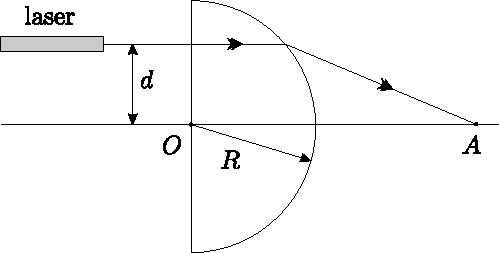
\includegraphics[width=0.8\linewidth]{2004-v3g-07-yl.pdf}
\end{center}

\hint

\solu
$d$ maksimaalse väärtuse määrab piirjuht, kus laserkiir langeb tagumisele pinnale täieliku sisepeegelduse piirnurga all, s.t. $\sin \alpha=1 / n$. Teiselt poolt, $\sin \alpha=d_{\max } / R$, seega $d_{\max }=R / n$.
\begin{center}
	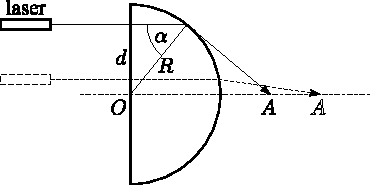
\includegraphics[width=0.8\linewidth]{2004-v3g-07-lah.pdf}
\end{center}
Kui $d=d_{\max}$, siis väljuv laserkiir on silinderpinnale puutujaks. Seega
$$
\begin{aligned}
	l &=R \cos \alpha+d_{\max } \tan \alpha=R\left[\sqrt{1-\sin ^{2} \alpha}+\frac{1}{n} \frac{\sin \alpha}{\sqrt{1-\sin ^{2} \alpha}}\right] \\
	&=R\left[\sqrt{1-1 / n^{2}}+\frac{1}{n} \frac{1 / n}{\sqrt{1-1 / n^{2}}}\right]=\frac{n R}{\sqrt{n^{2}-1}}
\end{aligned}
$$
Kui $d \rightarrow 0$, siis laserkiir langeb tagumisele pinnale nurga all $\alpha \approx d / R$. Murdumisnurk on $\beta=n \alpha=n d / R.$ Pinnanormaali kaldenurk on samuti $\alpha$, seega väljunud kiire kaldenurk on $\gamma=\beta-\alpha=(n-1) d / R$. Nüüd saame
$$
l=R+\frac{d}{\gamma}=R+\frac{R}{n-1}=\frac{n R}{n-1} .
$$

\probend